% \documentclass[12pt,english,ignorenonframetext,aspectratio=169,]{beamer}
\documentclass[11pt,english,ignorenonframetext,]{beamer}

%%%%%%%%%%%%%%%
%% Beamer theme
% choose one from http://deic.uab.es/~iblanes/beamer_gallery/
% or http://www.hartwork.org/beamer-theme-matrix/
% \usetheme{Warsaw}
\usetheme{CambridgeUS}

%%%%%%%%%%%%%%%%%%%%%%
%% Beamer color theme
%% default albatross beaver beetle crane dolphin dove fly lily
%% orchid rose seagull seahorse whale wolverine

%\usecolortheme{seahorse}  %% very lighty
\usecolortheme{dolphin}    %% nice blue
\usecolortheme{orchid}     %% dark red ?
\usecolortheme{whale}      %% black and blue as Warsaw

%%%%%%%%%%%%%%%%%%%%%%%%%%%%%%%%%%%%%%%%%%%%%%%%%%%%%%%%%%%%%%%%%%%%%%%%%%%%%%%%
%% Change the theme
%\setbeamercolor{alerted text}{fg=orange}
%\setbeamercolor{background canvas}{bg=white}
%\setbeamercolor{block body alerted}{bg=normal text.bg!90!black}
%\setbeamercolor{block body}{bg=normal text.bg!90!black}
%\setbeamercolor{block body example}{bg=normal text.bg!90!black}
%\setbeamercolor{block title alerted}{use={normal text,alerted text},fg=alerted text.fg!75!normal text.fg,bg=normal text.bg!75!black}
%\setbeamercolor{block title}{bg=blue}
%\setbeamercolor{block title example}{use={normal text,example text},fg=example text.fg!75!normal text.fg,bg=normal text.bg!75!black}
%\setbeamercolor{fine separation line}{}
\setbeamercolor{frametitle}{fg=black}
%\setbeamercolor{item projected}{fg=black}
%\setbeamercolor{normal text}{bg=black,fg=yellow}
%\setbeamercolor{palette sidebar primary}{use=normal text,fg=normal text.fg}
%\setbeamercolor{palette sidebar quaternary}{use=structure,fg=structure.fg}
%\setbeamercolor{palette sidebar secondary}{use=structure,fg=structure.fg}
%\setbeamercolor{palette sidebar tertiary}{use=normal text,fg=normal text.fg}
%\setbeamercolor{section in sidebar}{fg=brown}
%\setbeamercolor{section in sidebar shaded}{fg= grey}
\setbeamercolor{separation line}{}
%\setbeamercolor{sidebar}{bg=red}
%\setbeamercolor{sidebar}{parent=palette primary}
%\setbeamercolor{structure}{bg=black, fg=green}
%\setbeamercolor{subsection in sidebar}{fg=brown}
%\setbeamercolor{subsection in sidebar shaded}{fg= grey}
%\setbeamercolor{title}{fg=blackblue}
%\setbeamercolor{titlelike}{fg=blackblue}


%%%%%%%%%%%%%%%%%%%%%%%
%% Other beamer options
% \setbeamercovered{transparent}
\setbeamercovered{invisible}
% Permet de laisser en gris le texte qui n'est pas encore apparu (lorsqu'on utilise les commandes avec des <1,2> ou <4-9>.

%\setbeamercolor{normal text}{fg=black,bg=white}

%%%%%%%%%%%%%%%%%%%%%%%
%% Change Beamer fonts
% \usefonttheme{default}
% \usefonttheme[onlymath]{serif}
\usefonttheme{serif}

\setbeamerfont{title}{family=\rm}
\setbeamerfont{titlelike}{family=\rm}
\setbeamerfont{frametitle}{family=\rm}

%%%%%%%%%%%%%%%%%%%%%%%%%%%%%%%%%%%%%%%%%%%%%%%%%%%%%%%%%%%%%%%%%%%%%%%%%%%%%%%%
%% innertheme
%% rectangles circles inmargin rounded
% \useinnertheme{rounded}  % XXX My preference
\useinnertheme{circles}    % XXX

%%%%%%%%%%%%%%%%%%%%%%%%%%%%%%%%%%%%%%%%%%%%%%%%%%%%%%%%%%%%%%%%%%%%%%%%%%%%%%%%
%% outertheme
%% infolines miniframes shadow sidebar smoothbars smoothtree split tree
%\useoutertheme{infolines}

%% No navigation symbol.
\setbeamertemplate{navigation symbols}{}
\beamertemplatenavigationsymbolsempty

% XXX Add a background image to the slides
% \usepackage{tikz}
% \setbeamertemplate{background}{
\includegraphics[width=\paperwidth,height=\paperheight,keepaspectratio]{IETR.jpg}}
% \setbeamertemplate{background}{{\centering\begin{tikzpicture}\node[opacity=0.15]{
\includegraphics[width=0.98\paperwidth]{IETR_et_partenaires_IETR.png}};\end{tikzpicture}}}

% Other options
%\setbeamertemplate{footline}[page number]

\beamertemplateballitem
\setbeamertemplate{itemize item}[square]


\setbeamertemplate{caption}[numbered]
\setbeamertemplate{caption label separator}{: }
\setbeamercolor{caption name}{fg=normal text.fg}
\beamertemplatenavigationsymbolsempty
\usepackage{lmodern}
\usepackage{color}
  \newcommand{\urlb}[1]{\textcolor{blue}{\url{#1}}}
%% Color definition
\usepackage{xcolor}
%% WARNING attention when changing the colors, change both the {RGB}{r,g,b} and % rgb(r,g,b)
\definecolor{blackblue}{RGB}{19,19,59}  % rgb(48,48,150)
\definecolor{bleu}{RGB}{0,0,204}           % rgb(0,0,204)
\definecolor{deeppurple}{RGB}{102,0,204}   % rgb(102,0,204)
\definecolor{darkgreen}{RGB}{0,100,0}      % rgb(0,100,0)
\definecolor{yellowgreen}{RGB}{200,215,0}  % rgb(200,215,0)
\definecolor{bluegreen}{RGB}{0,185,140}    % rgb(0,185,140)
\definecolor{gold}{RGB}{255,180,0}         % rgb(255,180,0)
\definecolor{meca}{RGB}{255,110,0}         % rgb(255,110,0)
\definecolor{strongred}{RGB}{255,0,0}      % rgb(255,0,0)
\definecolor{normalred}{RGB}{204,0,0}      % rgb(204,0,0)
\definecolor{darkred}{RGB}{174,0,0}        % rgb(174,0,0)
\definecolor{info}{RGB}{174,0,0}        % rgb(174,0,0)
\definecolor{darkblue}{RGB}{0,0,174}        % rgb(0,0,174)
\definecolor{maths}{RGB}{0,0,174}        % rgb(0,0,174)
\definecolor{darkpurple}{RGB}{114,0,114}   % rgb(114,0,114)
\definecolor{ml}{RGB}{114,0,114}   % rgb(114,0,114)

\usepackage{amssymb,amsmath}
\usepackage{bbm,bm}  % bold maths symbols
\usepackage{ifxetex,ifluatex}
\usepackage{fixltx2e} % provides \textsubscript

% % FIXME remove as soon as possible, it slows down compilation to import TikZ
% %% TikZ
% \usepackage{tikz}
% \usetikzlibrary{snakes,arrows,shapes}
% % https://tex.stackexchange.com/a/226974/
% \tikzset{
%   font={\fontsize{10pt}{10}\selectfont}
% }
\usepackage{tikzsymbols}  % https://tex.stackexchange.com/a/227226/97964

\IfFileExists{macrosText.sty}{\usepackage{macrosText}}{}

\usepackage[linesnumbered,commentsnumbered,inoutnumbered,slide]{algorithm2e}


\ifnum 0\ifxetex 1\fi\ifluatex 1\fi=0 % if pdftex
  \usepackage[T1]{fontenc}
  \usepackage[utf8]{inputenc}
\else % if luatex or xelatex
  \ifxetex
    \usepackage{mathspec}
  \else
    \usepackage{fontspec}
  \fi
  \defaultfontfeatures{Ligatures=TeX,Scale=MatchLowercase}
\fi
% use upquote if available, for straight quotes in verbatim environments
\IfFileExists{upquote.sty}{\usepackage{upquote}}{}
% use microtype if available
\IfFileExists{microtype.sty}{%
\usepackage{microtype}
\UseMicrotypeSet[protrusion]{basicmath} % disable protrusion for tt fonts
}{}
\newif\ifbibliography
\hypersetup{
            pdfborder={0 0 0},
            breaklinks=true}
% \urlstyle{same}  % don't use monospace font for urls
% Code embedding.
\usepackage{palatino}              % Use the Palatino font % XXX remove if it is ugly ?
\usepackage{graphicx,grffile}
\makeatletter
\def\maxwidth{\ifdim\Gin@nat@width>\linewidth\linewidth\else\Gin@nat@width\fi}
\def\maxheight{\ifdim\Gin@nat@height>\textheight0.8\textheight\else\Gin@nat@height\fi}
\makeatother
% Scale images if necessary, so that they will not overflow the page
% margins by default, and it is still possible to overwrite the defaults
% using explicit options in \includegraphics[width, height, ...]{}
\setkeys{Gin}{width=\maxwidth,height=\maxheight,keepaspectratio}

\ifxetex
\usepackage{fontspec}
\setmainfont[Ligatures=Historic]{TeX Gyre Pagella}
\newfontfamily\FiraCode{Fira Code}
\setmonofont[Contextuals={Alternate}]{Fira Code}
\newfontfamily\Fontify[Path = ../common/]{Fontify-Regular}
\else
\newcommand{\Fontify}{}
\fi

% Prevent slide breaks in the middle of a paragraph:
\widowpenalties 1 10000
\raggedbottom

% \AtBeginPart{
%   \let\insertpartnumber\relax
%   \let\partname\relax
%   \frame{\partpage}
% }
% \AtBeginSection{
%   \ifbibliography
%   \else
%     \let\insertsectionnumber\relax
%     \let\sectionname\relax
%     \frame{\sectionpage}
%   \fi
% }
% % Si on veut faire apparaître le sommaire courant à chaque nouvelle section.
% \AtBeginSection{
%   \begin{frame}<beamer>%[t]
%   %\frametitle{Local outline}  % Translate the name of the slide
%   \frametitle{\hspace{0pt}}  % Translate the name of the slide
%     \begin{LARGE}  % XXX LARGE font for this slide?
%     \tableofcontents[currentsection, sectionstyle=show/hide, subsectionstyle=hide/hide]
%     \end{LARGE}  % XXX LARGE font for this slide?
%   \end{frame}
% }
% \AtBeginSubsection{
%   \let\insertsubsectionnumber\relax
%   \let\subsectionname\relax
%   \frame{\subsectionpage}
% }

\setlength{\parindent}{0pt}
\setlength{\parskip}{6pt plus 2pt minus 1pt}
\setlength{\emergencystretch}{3em}  % prevent overfull lines
\providecommand{\tightlist}{%
  \setlength{\itemsep}{0pt}\setlength{\parskip}{0pt}}
\setcounter{secnumdepth}{5}

% https://tex.stackexchange.com/a/70495/
\usepackage{appendixnumberbeamer}


% For \justifying command, see https://tex.stackexchange.com/a/148696/
\usepackage{ragged2e}
\addtobeamertemplate{frame begin}{}{\justifying}
\addtobeamertemplate{block begin}{}{\justifying}
\addtobeamertemplate{block alerted begin}{}{\justifying}
\addtobeamertemplate{block example begin}{}{\justifying}
\addtobeamertemplate{itemize body begin}{}{\justifying}
\addtobeamertemplate{itemize item}{}{\justifying}
\addtobeamertemplate{itemize subitem}{}{\justifying}
\addtobeamertemplate{itemize subsubitem}{}{\justifying}
\addtobeamertemplate{enumerate body begin}{}{\justifying}
\addtobeamertemplate{enumerate item}{}{\justifying}
\addtobeamertemplate{enumerate subitem}{}{\justifying}
\addtobeamertemplate{enumerate subsubitem}{}{\justifying}
\addtobeamertemplate{description body begin}{}{\justifying}
\addtobeamertemplate{description item}{}{\justifying}


\title[B-GLR test and Non-Stationary MAB]{The Bernoulli Generalized Likelihood Ratio test (B-GLR) for Non-Stationary Multi-Armed Bandits}
\subtitle{Research Seminar at PANAMA, IRISA lab, Rennes}

\author[Lilian Besson]{\Large \textbf{Lilian Besson}}

\institute[]{{\large
  PhD Student}{\newline
  \normalsize
  \newline SCEE team, IETR laboratory, CentraleSupélec in Rennes
  \newline \& SequeL team, CRIStAL laboratory, Inria in Lille}}

\date{Thursday $6^{\text{th}}$ of June, $2019$}

\begin{document}
\justifying

\begin{frame}[plain]
\titlepage

% XXX manual inclusion of logos
\begin{center}
  
\includegraphics[height=0.18\textheight]{../common/LogoIETR.png}
  
\includegraphics[height=0.21\textheight]{../common/LogoCS.png}
  
\includegraphics[height=0.18\textheight]{../common/LogoInria.jpg}
\end{center}

\end{frame}


\section{\hfill{}1. Présentation du candidat\hfill{}}

\subsection{\hfill{}Plan\hfill{}}

\begin{frame}{Outline of the talk}

\begin{enumerate}
\item
\alert{\textbf{%
  (Stationary) Multi-armed bandits problems
}}
\vspace*{15pt}

\item
\textcolor{gray}{
  Piece-wise stationary multi-armed bandits problems
}
\vspace*{15pt}

\item
\textcolor{gray}{
  The B-GLR test
}
\vspace*{15pt}

\item
\textcolor{gray}{
  The BGLRT-klUCB algorithm
}
\vspace*{15pt}

\item
\textcolor{gray}{
  Regret analysis
}
\vspace*{15pt}

\item
\textcolor{gray}{
  Numerical simulations
}
\end{enumerate}

\end{frame}


\begin{frame}{Associated publications}

\begin{itemize}
\item
  \href{https://hal.inria.fr/hal-02006471/document}{``Analyse non asymptotique d'un test séquentiel de détection de ruptures et application aux bandits non stationnaires''}, by \textbf{L. Besson} \&
  \href{http://chercheurs.lille.inria.fr/ekaufman/research.html}{E.
  Kaufmann}.
  \textbf{GRETSI}, Lille, France, August 2019

\end{itemize}

\begin{itemize}

\item
  \href{https://hal.inria.fr/hal-02006471/document}{``The Generalized Likelihood Ratio Test meets klUCB: an Improved Algorithm for Piece-Wise Non-Stationary Bandits''}, by \textbf{L. Besson} \&
  \href{http://chercheurs.lille.inria.fr/ekaufman/research.html}{E.
  Kaufmann}, February 2019,
  \href{https://hal.inria.fr/hal-02006471}{HAL-02006471}.

\end{itemize}

\end{frame}


% \subsection{\hfill{}Démonstration d'un problème de bandit\hfill{}}

\begin{frame}{Bandits multi-bras}

  Prise de décisions séquentielles face à un environment incertain

  \centering
  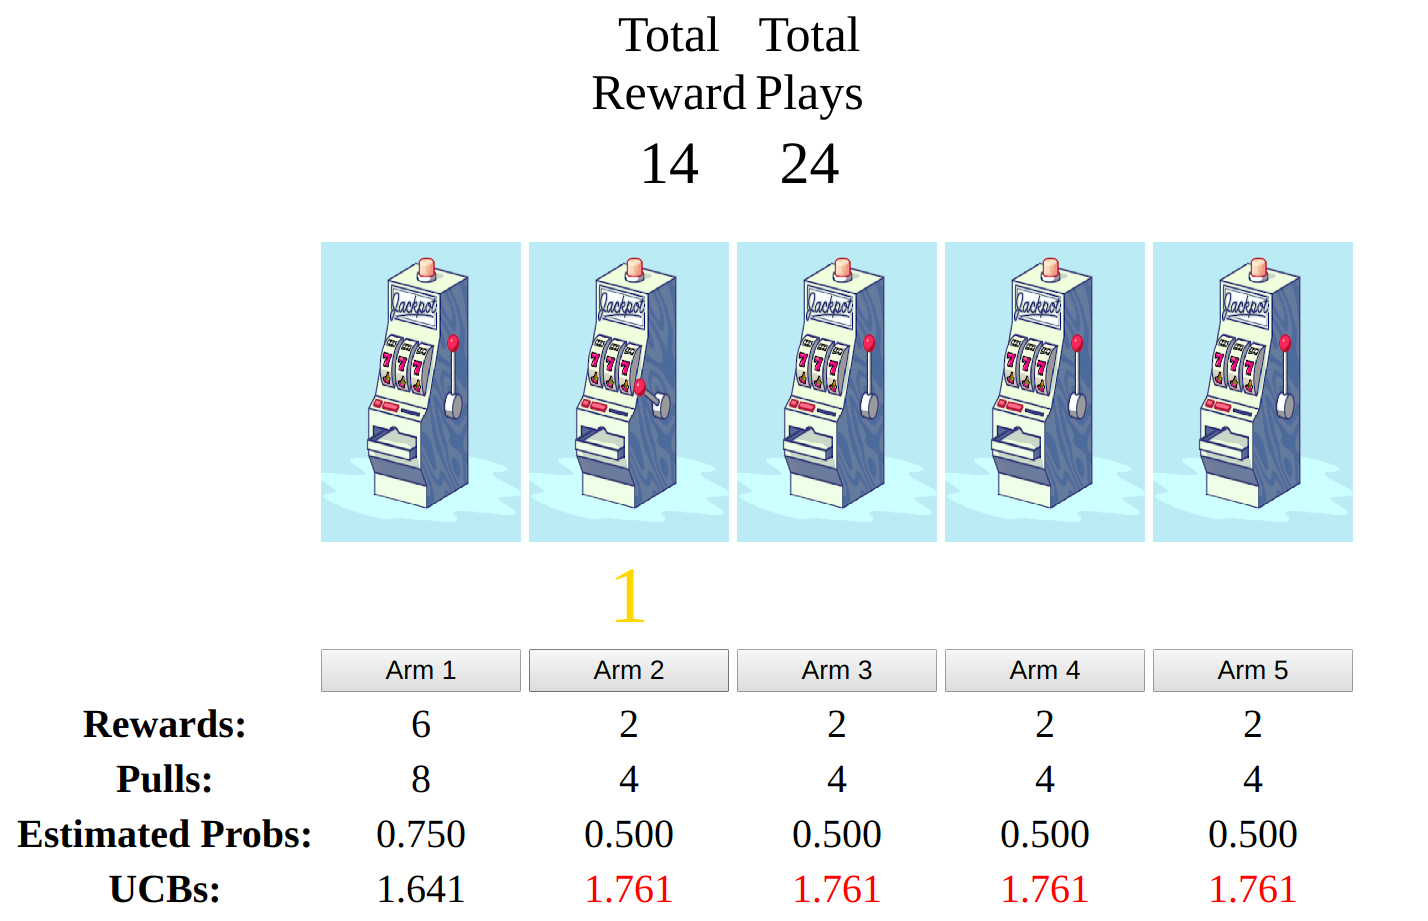
\includegraphics[height=0.65\textheight]{figures/example_of_a_5_arm_bandit_problem.png}

  {\tiny
      $\hookrightarrow$ \href{https://perso.crans.org/besson/phd/MAB_interactive_demo/}{\textcolor{blue}{\texttt{perso.crans.org/besson/phd/MAB\_interactive\_demo/}}}
  }

\end{frame}


\subsection{\hfill{}Algorithme \emph{``Upper Confidence Bound''}\hfill{}}

\begin{frame}{Exemple de solution : l'algorithme UCB}

Au temps $t$, on joue le bras $C(t)\in\{1,\dots,K\}$, on observe la récompense \emph{iid} aléatoire $r(t) \sim \mathrm{Bernoulli}(\mu_k) \in\{0,1\}$.
But : maximiser $\sum\limits_{t=1}^T r(t)$

\pause
\begin{itemize}
  \item
  Compter le nombre d'échantillons et la somme des récompenses pour chaque bras
  % \item
  % Et la somme des récompenses
  \[
    N_k(t) := \sum\limits_{s < t} \bold{1}(C(s)=k),
    \;\;\;\;
    X_k(t) := \sum\limits_{s < t} r(s) \bold{1}(C(s)=k)
  \]
  \pause
    \item
  Calculer $\mathrm{UCB}_k(t) = X_k(t) / N_k(t) + \sqrt{\alpha \log(t) / N_k(t)}$ \\
  $=$ une borne supérieure de confiance sur la moyenne $\mu_k$ \alert{inconnue}
  \item
  Jouer le bras d'UCB maximum : $C(t) = \arg\max_k \mathrm{UCB}_k(t)$
  % \\
  % $\hookrightarrow$ Principe d'optimisme face à l'incertain
    \item
  % $\alpha$ contrôle l'
  Équilibre entre \emph{exploitation} ($\alpha\to0$) et \emph{exploration}  ($\alpha\to\infty$)
\end{itemize}

\end{frame}


% \subsection{\hfill{}Mesure de performance pour les algorithmes de bandits\hfill{}}

\begin{frame}{Mesurer la performance d'un algorithme $\mathcal{A}$ avec son regret (moyen) $R_{\mathcal{A}}(T)$}

\pause

\begin{itemize}
  \item
  Différence de récompenses accumulées entre un ``oracle'' et $\mathcal{A}$

  \item
  L'algorithme ``oracle'' joue le meilleur bras $k^* = \arg\max \mu_k$

  \item
  Maximiser les récompenses cumulées
  $\Longleftrightarrow$ \alert{minimiser le regret}
  %
  \[ \alert{ R_{\mathcal{A}}(T) } := \mathbb{E}\left[ \sum\limits_{t=1}^T r_{k^*}(t) \right] - \sum\limits_{t=1}^T \mathbb{E}\left[ r(t) \right] = T \mu_{k^*} - \sum\limits_{t=1}^T \mathbb{E}\left[ r(t) \right]. \]

\end{itemize}

\pause
\vspace*{10pt}

\begin{exampleblock}{Régime typique pour des problèmes stationnaires (borne inf \& sup)}
  \begin{itemize}
  \item
  Aucun algorithme ne peut obtenir mieux que
  \hfill{}
  $R_{\mathcal{A}}(T) \geq \Omega(\log(T))$

  \item
  Et un algorithme efficace $\mathcal{A}$ obtient
  \hfill{}
  $R_{\mathcal{A}}(T) \leq \mathcal{O}(\log(T))$
  \end{itemize}
\end{exampleblock}

\pause

\begin{exampleblock}{Exemple de borne de regret : pour l'algorithme UCB}
  Pour tout problème avec $K$ bras distribués selon des lois de Bernoulli, de paramètres $\mu_1,\dots,\mu_K \in[0,1]$, de bras optimal $k^*$
  \begin{small}
    \[ R_T^{\mathrm{UCB}} \leq \left( \sum_{\substack{k=1,\dots,K \\ \mu_k < \mu_{k^*}}} \frac{8}{(\mu_k - \mu_{k^*})^2} \right) \log(T) + o(\log(T)) = \mathcal{O}\left( \alert{C(\mu_1,\dots,\mu_K)} \log(T) \right). \]
  \end{small}%
\end{exampleblock}

\end{frame}


% \begin{frame}{Contributions principales de ma thèse}
\begin{frame}{Deux contributions principales de ma thèse}

Pour différentes extensions du modèle classique de bandits\ldots{}

\begin{itemize}
  \item
  Formalisation mathématique
  \item
  Nous proposons de nouveaux algorithmes\ldots{}
  % \item
  \newline
  avec une nouvelle analyse théorique, nouvelles bornes de regret\ldots{}
  % \item
  \newline
  validées par des simulations numériques\ldots{}
  \item
  $\implies$ Améliore l'état de l'art sur les deux aspects !
\end{itemize}

\end{frame}


\begin{frame}{Deux contributions principales de ma thèse}

\begin{exampleblock}{Bandits stationnaires (classiques) avec $K$ bras et $T$ étapes}
  \[ R_{\mathcal{A}}(T) = \mathcal{O}\left( K \log(T) \right). \]
\end{exampleblock}

\begin{block}<2->{1) Bandits \textbf{multi-joueurs décentralisé} \hspace*{40pt} \href{https://arxiv.org/abs/1711.02317}{[Besson et al, ALT, 2018]}}
  Si \alert{$M \leq K$ joueurs} jouent face au même problème de bandit, \alert{avec collisions} mais sans communication entre eux ni sans contrôle centralisé :
  %
  $R_{\mathrm{MCTopM}}(T) = \mathcal{O}\left( K \alert{M^3} \log(T) \right)$.
\end{block}

\begin{block}<3->{2) Bandits stationnaires \textbf{par morceaux} \hspace*{25pt} \href{https://arxiv.org/abs/1902.01575}{[Besson et al, GRETSI, 2019]}}
  Si le problème est \alert{stationnaire par morceaux, sur $\Upsilon = o(\sqrt{T})$ intervalles ``assez grands''} :
  %
  $R_{\mathrm{B}\text{-}\mathrm{GLR}}(T) = \mathcal{O}\left( K \sqrt{\alert{\Upsilon} T \log(T)} \right)$.
\end{block}

\end{frame}



\begin{frame}[plain]{\normalsize Simulations d'algorithmes de bandits \alert{non stationnaires} avec ma bibliothèque SMPyBandits, écrite en Python \hfill{}\textcolor{gray}{[Besson et al, GRETSI, 2019]}}

  \centering
  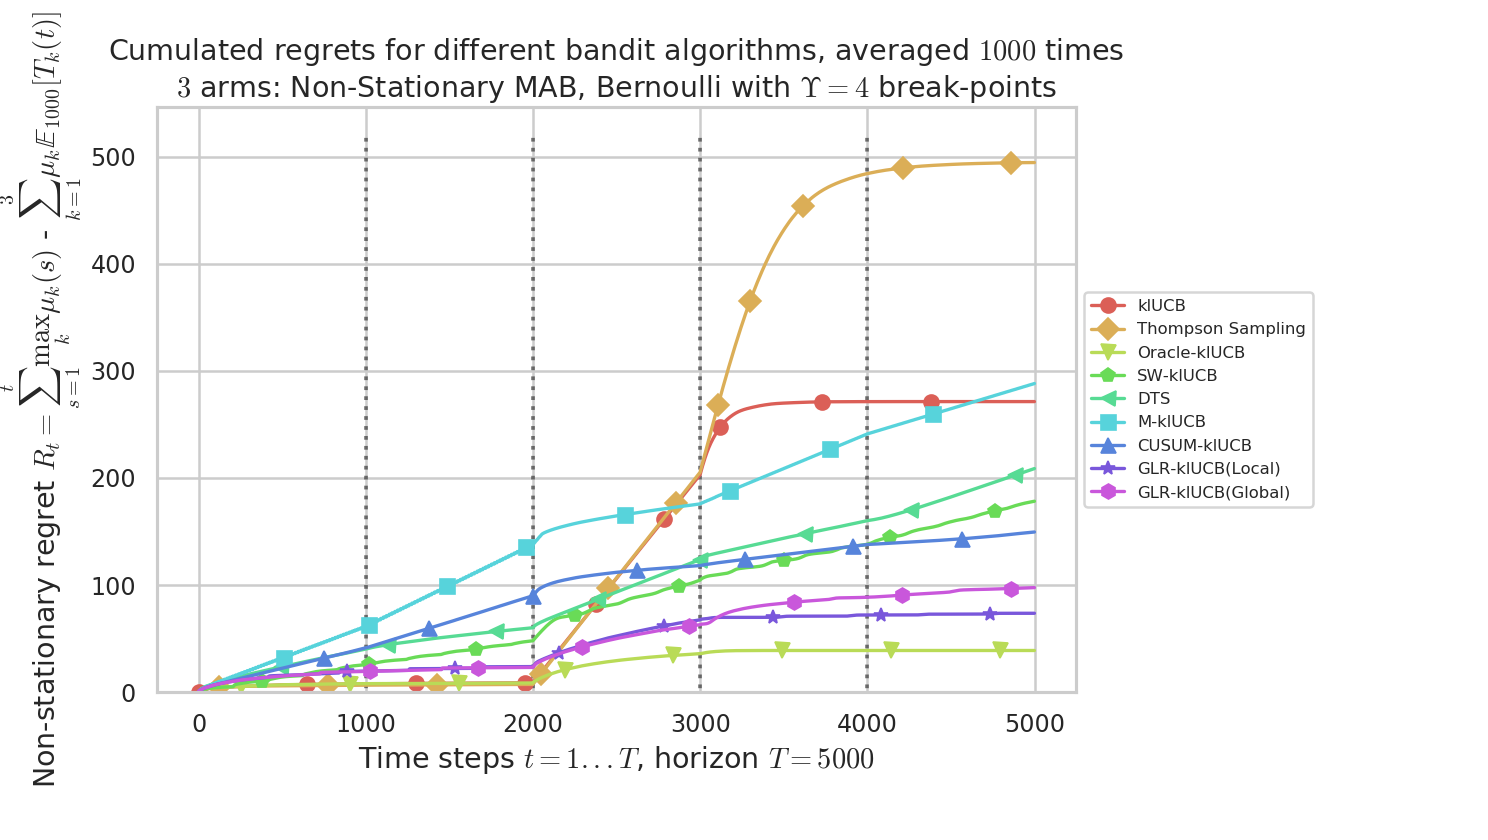
\includegraphics[width=1.15\textwidth]{figures/example_regret_non_stationary_bandits.png}

\end{frame}



\section{\hfill{}Conclusion\hfill{}}
\subsection{}

\begin{frame}{Conclusion}

\begin{center}
  \begin{Large}
    {\Fontify Thanks for your attention .}
    \Smiley[0.9]
  \end{Large}
\end{center}

\begin{center}
  \begin{Large}
    Questions \& discussion
  \end{Large}
\end{center}

\end{frame}

\end{document}
